\section{Wprowadzenie}

Związki nasycone: alkany, cykloalkany

Związki nienasycone: alkany, alkiny, aromatyczne, cykloalkeny, enyny
\newline

Enyny- zawierają wiązanie podwójne i potrójne [numerację zaczynamy od bliższego bądź gdy są w tej samej odległości to od podwójnego].
\newline

Węglowodory alifatyczne- wszystkie związki organiczne niearomatyczne (również te o łańcuchach zamkniętych).
\newline

\begin{figure}[H]
    \centering
    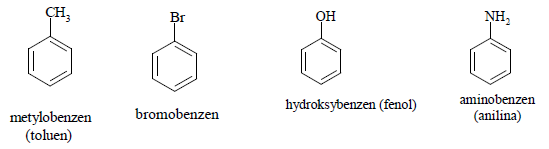
\includegraphics[width=0.7\textwidth]{img/benzeny}
    \label{fig.benzeny}
\end{figure}

\begin{figure}[H]
    \centering
    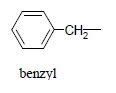
\includegraphics[width=0.2\textwidth]{img/benzyl}
    \label{fig.benzyl}
\end{figure}

\begin{figure}[H]
    \centering
    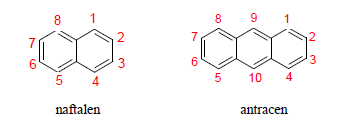
\includegraphics[width=0.7\textwidth]{img/naftalen}
    \label{fig.naftalen}
\end{figure}